\subsection{2021年3月1日}
\paragraph{\href{https://www.51voa.com/VOA_Special_English/new-study-black-hole-may-be-larger-than-expected-86383.html}{原文}}

\begin{figure}[H]
\centering
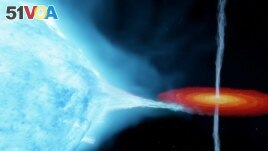
\includegraphics[scale=0.7]{005_voa_20210301.jpg}
\caption{FILE - An artist's impression of the Cygnus X-1 system, with a so-called stellar-mass black hole orbiting a companion star some 7,200 light years from Earth. (International Centre for Radio Astronomy Research/Handout via REUTERS)}
\end{figure}

By John Russell
27 February 2021
A recent study found that the first black hole ever discovered is a lot bigger than scientists first thought.
Black holes are extremely massive space objects whose gravity is so powerful not even light escapes. The black hole, Cygnus X-1, was discovered in 1964. It is well-known for being the object of a friendly bet between two famous scientists.
Researchers found that new observations of Cygnus X-1 showed it is 21 times our sun's mass. That is about 50 percent more massive than scientists had believed.
While it is still one of the closest black holes known, the scientists found it is farther away than earlier estimates suggested. It is 7,200 light years away. A light year is the distance light travels in one year.
Some black holes, like the one at the center of the Milky Way Galaxy, are extremely large. These are called "supermassive" black holes. They can be millions of times more massive than the sun. Smaller black holes are called "stellar-mass" black holes. They have the mass of a single star.
Cygnus X-1 is the Milky Way's largest-known stellar-mass black hole. It is among the strongest X-ray sources seen from Earth, said James Miller-Jones of Curtin University and the International Centre for Radio Astronomy Research in Australia. Miller-Jones led the study that appeared in the publication Science.
Cygnus X-1 turns so quickly that it comes close to the highest rate predicted under physicist Albert Einstein's theory of general relativity, Miller-Jones added.
The black hole brings in material that comes from the surface of the star that it orbits. This star is a "blue supergiant," a very large star about 40 times our sun's mass.
Cygnus X-1 started to exist 4 million to 5 million years ago as a star up to 75 times more massive than the sun. But then it collapsed into a black hole a few tens of thousands of years ago.
The research included data from the Very Long Baseline Array radio telescope. It is made up of 10 observation stations in the United States.
After Cygnus X-1 was first identified as a possible black hole, a friendly bet was made between two physicists, Stephen Hawking and Kip Thorne. Hawking bet against the object being a black hole, while Thorne bet that it was one. Hawking eventually admitted that the evidence suggested Cygnus X-1 was a black hole.
Miller-Jones, the leader of the recent study said, "Indeed, I did not have any wagers riding on these findings."
I'm John Russell.
Will Dunham reported on this story for Reuters. John Russell adapted it for Learning English. Mario Ritter, Jr. was the editor.

\begin{messagebox}
Words in This Story
bet – n. an agreement in which people try to guess what will happen and the person who guesses wrong has to give something (such as money) to the person who guesses right; a wager
source – n. the place where something starts from
wager – n. an agreement in which people try to guess what will happen and the person who guesses wrong has to give something (such as money) to the person who guesses right; a bet
\end{messagebox}

A recent study found that the first black hole ever discovered is a lot bigger than scientists first thought.
一项最新研究发现,人类有史以来发现的第一个黑洞要比科学家最初认为的要大得多。
Black holes are extremely massive space objects whose gravity is so powerful not even light escapes. The black hole, Cygnus X-1, was discovered in 1964. It is well-known for being the object of a friendly bet between two famous scientists.
黑洞是极其巨大的空间物体,其引起是如此之大,甚至连光都无法逃脱。天鹅座X-1黑洞于1964年被发现。它因为成为两位科学家之间友好打赌的对象而闻名。
Researchers found that new observations of Cygnus X-1 showed it is 21 times our sun's mass. That is about 50 percent more massive than scientists had believed.
研究人员发现,对天鹅座X-1的新观测表明其质量是太阳系的21倍。这比科学家之前认为的要大50%。
While it is still one of the closest black holes known, the scientists found it is farther away than earlier estimates suggested. It is 7,200 light years away. A light year is the distance light travels in one year.
尽管它仍然是已知最接近地球的黑洞之一,但是科学家们发现它比之前估计的要远得多。它距离我们有7200光年。1光年是指光在1年当中传播的距离。
Some black holes, like the one at the center of the Milky Way Galaxy, are extremely large. These are called "supermassive" black holes. They can be millions of times more massive than the sun. Smaller black holes are called "stellar-mass" black holes. They have the mass of a single star.
有些黑洞非常大,例如银河系当中的黑洞。这些被称之为“超大质量”黑洞。它们的质量可能是太阳的几百万倍。较小的黑洞被称为恒星级黑洞。它们具有单颗恒星的质量。
Cygnus X-1 is the Milky Way's largest-known stellar-mass black hole. It is among the strongest X-ray sources seen from Earth, said James Miller-Jones of Curtin University and the International Centre for Radio Astronomy Research in Australia. Miller-Jones led the study that appeared in the publication Science.
天鹅座X-1是银河系当中最大的恒星级黑洞。科廷大学和澳大利亚国际射电天文学研究中心的詹姆斯·米勒琼斯说,这是从地球上观测到的最强的X射线源之一。米勒琼斯领导了这项研究,其研究结果发表在《科学》杂志上。
Cygnus X-1 turns so quickly that it comes close to the highest rate predicted under physicist Albert Einstein's theory of general relativity, Miller-Jones added.
米勒琼斯还说,天鹅座X-1的自转是如此之快,以至于接近物理学家爱因斯坦的广义相对论所预测的最高速度。
The black hole brings in material that comes from the surface of the star that it orbits. This star is a "blue supergiant," a very large star about 40 times our sun's mass.
这个黑洞吸取了它所绕行的恒星表面的物质。这颗恒星是蓝巨星, 它是一颗非常巨大的恒星,其质量约为太阳质量的40倍。
Cygnus X-1 started to exist 4 million to 5 million years ago as a star up to 75 times more massive than the sun. But then it collapsed into a black hole a few tens of thousands of years ago.
天鹅座X-1的存在始于400万到500万年前,它是一颗质量是太阳75倍的恒星。但是在几万年前,它坍塌成了一个黑洞。
The research included data from the Very Long Baseline Array radio telescope. It is made up of 10 observation stations in the United States.
这项研究包含的数据来自于甚长基线射电望远镜阵。它是由美国的10个观测站组成的。
After Cygnus X-1 was first identified as a possible black hole, a friendly bet was made between two physicists, Stephen Hawking and Kip Thorne. Hawking bet against the object being a black hole, while Thorne bet that it was one. Hawking eventually admitted that the evidence suggested Cygnus X-1 was a black hole.
在天鹅座X-1最初被认定可能是黑洞之后,斯蒂芬·霍金和基普·索恩这两位物理学家进行了一项友好的打赌。霍金赌这个物体不是黑洞,而索恩赌那就是一个黑洞。霍金最终承认,有证据表明天鹅座X-1是一个黑洞。
Miller-Jones, the leader of the recent study said, "Indeed, I did not have any wagers riding on these findings."
这项最新研究的负责人米勒琼斯表示:“其实我对这些发现没投任何赌注。”
